% $Id: compnames.tex 8161 2009-04-06 14:07:39Z alexandra $
% Local Variables:
% ispell-check-comments: nil
% Local IspellDict: american
% End:
% --------------------------------------------------------
% User documentation
% copyright by BREDEX GmbH 2004
% --------------------------------------------------------
\index{Component!Names!Reassigning}
\index{Reassigning!Component Names}
\index{View!Component Names}
\index{Component!Names!View}
\index{Names!Component!Reassigning}
 \label{reassconcepts}
Once you have made your \gdcases{} reusable, you can add them to other \gdcases{}. 
The  component names you use can be \bxname{reassigned} when you reuse the \gdcase{} they are in. 

This creates a new name for the component in the \gdomeditor{}, which can then be mapped to another component in the \gdaut{}. This means that you can use one \gdcase{} to test the same action on different components. So you can specify one \gdcase{} to click a button, and use it every time you want your test to click a button in the \gdaut{}.

%\bxtipp{You can only map components of the same type as the original name}

If you use abstract components, you increase the amount of components your \gdcase{} can be mapped to, which reduces redundancy and makes the test easier to maintain. 

As with references, you can move component names one level up in the hierarchy by checking the box in the \gdcompnamesview{}. This means that the component name can also be overwritten at the next level, when that \gdcase{} is reused.  

\begin{figure}
\begin{center}
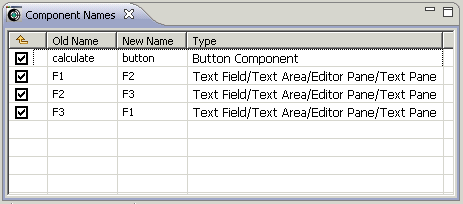
\includegraphics{Concepts/PS/compnames}
\caption{\gdcompnamesview}
\label{compnames}
\end{center}
\end{figure}



